\chapter{System Design}\label{ch:setup}

In this chapter we discuss the overall system design of the project.
First, we provide an architectural overview
of the system and the various components in \cref{sc:architectural-overview}.
We then discuss the requirements of the system from the user's point of view
(\cref{sc:real-user}), from the cryptographic point of view
(\cref{sc:abstract-to-real}) and from the developer's point of view
(\cref{sc:developer}). We highlight the importance
of taking into account all points of view and stress the 
relevance of considering the real-world
user for the choice of technologies in the implementation. 

After laying out the requirements, we discuss the various
components of the system, detailing for each of them
the technology we use. In-depth technical
discussion and technology surveys are provided
to motivate our final choice when required, and we believe
that this is of great interest to the practitioners
that want to implement cryptographic systems with 
a similar technology stack.\footnote{The term ``technology stack'' (or tech stack) generally refers to the set of technologies used together to build a software product.}
However, the reader should feel free to safely skip
them, as they are not strictly necessary to understand 
the rest of this work.

We only discuss common
pieces to both the baseline and the SSF implementation
in this chapter. Most of the system is
shared between the two implementations, to allow
for easy comparison and benchmarking.
The specifics of each implementation are instead discussed respectively in \cref{ch:baseline,ch:ssf}.

\section{Architecture Overview}\label{sc:architectural-overview}

In figure \cref{fig:architecture} we provide a high-level system architecture overview.
We use different colours to highlight different components of the system, grouping
by frontend, backend, relational databases and cloud components.

\paragraph{Client} The SSF client is a web application that
runs in the browser. The client is used by the user to interact with the system, and performs the cryptographic
operations needed to access, store and retrieve files 
from the shared folders the user has access to.
Although in the \cref{sc:SSF-scheme} we only model one folder,
in practice the system supports multiple ones.
We imagine the final version of the user interface (UI) to
be similar to the one of Google Drive or Dropbox, where
the user can see the shared folders and navigate inside each
of them to see a list of files stored in each of them.
The UI is out of scope from this project, due to
time constraints (\cref{sc:client-overview}), we will
instead provide a command line interface (CLI) client
as MVP.

\paragraph{PKI} The system needs a PKI to manage the identities
of its users. We assume a corporate environment, where
an internal identity provider is available. The PKI server
is a simple certificate authority (CA) which is trusted
by the clients, and issues certificates to users of the system.
The CA certificate is generated once and embedded in the client
code to allow for the verification of other users' certificates.
All the certificates are stored in a relational SQL database \texttt{pki}.

\paragraph{SSF Gateway and DS}
The SSF Gateway server is the main backend component of the system.
The same server will be used also to implement a delivery service (DS) (see \cref{sc:MLS} and \cref{ssc:delivery-service}).
These are two different components in abstract, but in practical terms, 
we will see that they share some state (\cref{ssc:delivery-service}).
The SSF Gateway, or simply Gateway, is responsible for the
creation of the shared folders (\cref{sc:SSF-scheme}) and the management of user access
to them. The shared folders are stored in a relational SQL
database \texttt{ds}, together with the users access control lists (ACLs).
Since different cloud storage providers offer different APIs,
the Gateway is responsible for abstracting away the specific
vendor and providing a common API to the clients.
Through the Gateway, files can be uploaded and downloaded 
from the cloud storage provider, which is hidden from the client,
as can be seen in \cref{fig:architecture}.
We can imagine, that the Gateway would constitute the main
server of a company offering a service for secure file sharing.

\begin{figure}
    \centering
    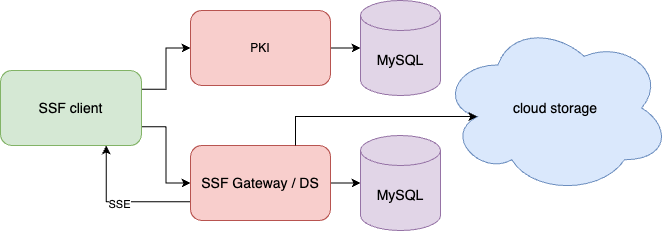
\includegraphics[width=0.8\textwidth]{figures/architecture.png}
    \caption{System Architecture Overview: The main components of the system are shown with the dependencies between them.}
    \label{fig:architecture}
\end{figure}

\section{High-Level Practical Requirements}\label{sc:requirements}

After this initial very high-level overview of the system, we
now move on to discuss its requirements instead and continue with a more
detailed explanation of the components of the system in the following sections.
This should motivate some of the choices we made in the architecture,
and be the background for the following detailed description.

\subsection{Starting with the User in Mind}\label{sc:real-user}

A goal of this thesis (\cref{sc:summary-of-contributions})
is to create an MVP. To this end, we start by asking ourselves,
as users of the system, what do we want from it?
\footnote{The study of the use cases and situations from a product 
point of view in industry is normally done through so-called ``user stories''.
User stories as sentences that try to summarise a workflow from the
point of view of a user. They have the following structure:
``As [a user persona] I want [to perform this action] so that [I can accomplish this goal]''.}
Our exploration is limited in time therefore we want to simplify
our requirements to the minimum necessary to run the system
in a real-world setting, 
but still with a customer-centric\footnote{To be customer-centric is a famous Amazon core approach. Indeed, Amazon has a leadership principle called ``customer obsession''~\cite{AmazonLeadershipPrinciples}.}
approach, leaving the possibility to iterate over the initial implementation~\cite{ries2011startup}.
We stress that we do not want to develop just a proof-of-concept of the protocol,
but something practically deployable and scalable to a large
amount of users.

As users, we expect to be able to access 
cloud systems from any device that can navigate online.
This is indeed a core minimum requirement for any modern
cloud storage solution for market adoption.
We also think this is a challenge that is worth exploring
in the context of SSF to understand if the underlying
schemes (\cref{ssc:GKP-client-middleware} \cref{sc:background-generalised-DKR})
are feasible and applicable for real use cases.
Normally, such ubiquitous access to cloud storage solutions,
is through a web interface.
This in turn means that we need to run our code (at least a part of it) 
in the browser of the user.

Other user expectations include updates and changes to uploaded files.
Further, we expect our system to provide multi-tenancy,
meaning that we handle multiple groups of users at the same time.\footnote{Note that each shared folder is in a one-to-one relationship with the group of users that have access to it.} 
Another side of the multi-tenancy aspect is that a 
single user could be part of multiple such groups at once. 
However, we point out that the SSF scheme (\cref{sc:SSF-scheme}) 
itself is designed for a single shared folder at the time.
Indeed, the underlying primitive GKP (\cref{sc:gkp-scheme}) focus 
on one group at a time in an isolated execution environment:
it is therefore up to our implementation to fill this gap.

We highlight that all major (non-E2EE) file sharing solutions available today meet the above requirements.
Therefore, we claim that these requirements and expectations should be met by any serious attempt to create a new cloud storage solution, including the implementation of the SSF scheme.\footnote{A notable exception is Apple's Advanced Data Protection, which is not accessible via web browser. This is partially thanks to the high level of integration of Apple hardware and software.}

\subsection{Cryptography: from Math to Real Execution Environments}\label{sc:abstract-to-real}

Before writing any code, we need to choose the right 
programming language that targets the execution environment
we want to run the code in.

As seen in \cref{ch:background}, the SSF scheme (\cref{sc:SSF-scheme})
uses some advanced cryptographic primitives:
\begin{itemize}
    \item continuous group key agreement (CGKA) (\cref{sc:CGKA})
    \item seekable sequential random generators (SSKG) (\cref{sc:SSKG})
    \item dual-key regression (DKR) (\cref{sc:background-generalised-DKR})
    \item group key progression (GKP) (\cref{sc:gkp-scheme})
\end{itemize}
Implementing these primitives from scratch could in itself
be a complex, time-consuming and error-prone task, especially for CGKA.
It is therefore important to use libraries when available
to deliver reliable implementations.

In our execution environment 
we need support for all cryptographic operations
needed both by the primitives above and by simpler
cryptography which is normally exploited and assumed to exist. 
To be more precise we require:
\begin{itemize}
    \item Secure random number generation.
    \item Availability and constant time execution of the cryptographic operations underlying the constructions we implement, both for the baseline and the SSF scheme.
    \item Memory safety.
\end{itemize}
The above requirements are needed to avoid security
issues in the implementation. For example, a non-constant
time execution of the cryptographic operations could
lead to timing attacks. 
However, during our implementation work, 
we found that in major runtime
environments, such as the browser, 
support for the cryptographic operations normally
used to instantiate cryptographic primitives is not always available.
This might lead to the usage of custom implementation,
where such guarantees are impossible to provide because
of the lack of low-level control on the execution environment.
We detail such findings throughout the rest of the thesis,
and summarise them among other engineering issues in \cref{ch:gaps}.

\subsection{What does the Developer need?}\label{sc:developer}

As developers, we face the challenge of implementing a full
system in a very short time frame and with limited resources.\footnote{To be more precise, the whole implementation has been conducted by only one person in less than six months.}
We want to reduce the possibility of errors and bugs
as well as the complexity of maintaining the integration between
different components.
Sometimes, just a small change in the protocol can lead to
hundreds of lines of changes in the code.
Even more, we want to be able to easily prototype, i.e.\ test
out different ideas coming from the theoretical side
or different engineering solutions.
However, changing requirements during the implementation
and updating the system accordingly can take up months of work
if the setup is not properly done to allow development agility.
We will see how this is achieved in the description of the various components.


\section{The PKI}\label{sc:PKI}

This section presents the PKI server implementation from the architecture overview (\cref{sc:architectural-overview}).

Recall from \cref{sc:mental-model} that
we need a Public Key Infrastructure (PKI) to implement the SSF scheme.
Papers in cryptography normally assume the existence of a PKI,
which solves the problem of mapping identities to cryptographic keys.
Since we want to develop the code easily, and the PKI itself
is not the core problem we are focusing on, we want to rely on existing
solutions.
A common standard way to manage identities is through X509 certificates~\cite{rfc5280}.
To implement this solution, we need to have a Certificate Authority (CA)
to distribute the certificates.
Our MVP target use case is a company or organization. 
Thus, we can assume to have an internal identity provider.
We implement a simple CA, with an endpoint for users
to register and one to fetch users' certificates. 
Users send certificate signing requests to be signed by the CA to register.
The CA certificate is bundled with the client code, to
allow the verification of other users' certificates.
The endpoints of the PKI are secured through TLS,
while the SSF Gateway will use mutual TLS (\cref{sc:ssf-proxy-server}).
We highlight that this PKI server implementation is not meant for production use:
for instance, we implement our CA purely in software, while a production
version would need to support hardware security mechanisms to
store secret key material.


\paragraph{Implementation Details} 
The PKI server is implemented in Rust, using \texttt{Rocket}~\cite{Rocket}
framework for the server and \texttt{sqlx} driver to interact
with the MySQL database.
In the early exploration of the project, we tried
to use other Rust web development frameworks,
such as \texttt{Actix}~\cite{Actix} and \texttt{Warp}~\cite{Warp}.
However, we found that \texttt{Rocket} was the most
suitable for our needs (see also \cref{sc:ssf-proxy-server}),
thanks to its support for retrieving the certificate
from the request when mTLS is used.
As we want to minimise the development overhead, we
try to reuse frameworks and libraries as much as possible. 

For local development, 
the database runs in a Docker container, which allows
for easy setup and teardown.\footnote{Docker is a lightweight virtualization technology. Docker containers are equivalent to lightweight virtual machines, but access the host's kernel rather than perform full CPU and IO virtualization.} 
The database is initialised with the script \texttt{sql/pki\_database.sql}.
It is important to have the ability
to easily reset the database to a fresh state 
while developing and testing the system.
The commands to start and stop the container are provided
in the top level \texttt{README.md} of the project.

The code is available in the \texttt{pki} crate
of this project, in \texttt{services/pki} folder.\footnote{``Crate'' is the name for a Rust package.}
The server exposes a simple API
to issue certificates to users. 
When issuing a certificate, validation is not performed
on the user identity, as this is out of scope for the MVP.
A client can send a certificate signing request (CSR)
to the server and receive a signed certificate in return.
The signing algorithm is ECDSA using P-256 curves and SHA-256 hashing
as described in~\cite{rfc5758}.
The code to construct the CSR and issue certificates, as well as 
verify them is available in the Rust crate \texttt{common},
which is shared among servers and clients (\cref{sc:client-overview}).
We provide unit tests for the library and expose simple bindings (\cref{sc:browser-runtimes}) to be
called from JavaScript in the client (\cref{sc:client-overview}), check the \texttt{README.md}
of the crate for details. All the exposed functionalities are stateless.

The certificates are stored in MySQL ``pki'' database, and the CA
certificate is copied and embedded in the client code to allow
for local verification of other users' certificates.
The server exposes an endpoint to fetch the
CA certificate, which can be used by clients to
refresh the embedded CA certificate.
Further, an endpoint to fetch users' certificates providing the email of the target user is available.
The description of how to compile and start the server is
provided in the \texttt{README.md} file of the \texttt{pki} crate.
The server is exposed locally at \texttt{\url{https://localhost:8000}}



\paragraph{OpenAPI Specification}
The server API is available in OpenAPI
specification format~\cite{OpenAPISurvey} 
which is generated automatically from the code using
\texttt{utoipa}. Each server endpoint code is
annotated through the library annotations, with the description
of the endpoint, parameters etc. \texttt{utoipa} is then
able to generate the OpenAPI specification in YAML format.
We store the generated file in \texttt{openapi/pki-openapi.yaml}.
We provide an executable written in Rust to perform the generation
through \texttt{utoipa} and regenerate the \texttt{.yaml}
file when the server endpoints are modified.
The OpenAPI specification is then used to generate the
code in TypeScript, which is used by the client to interact
with the PKI server (\cref{sc:client-overview}), thus sparing
the developer from writing thousands of lines of code and keeping them up to date, 
as well as reducing the possibility of errors in the client-server interaction. 
The guide on how to use the executable can be found in the \texttt{README.md}
of the crate.
While the server is running, the OpenAPI specification can be
accessed nicely through the Swagger UI from the browser, 
by visiting the page \texttt{\url{http://localhost:8000/swagger/UI}}.

\section{Cloud Storage: from an Abstract Model to Real Systems}\label{sc:cloud-storage}

This section provides the necessary background on cloud storage,
aiming to provide the reader with a first understanding of the challenges
we encounter when dealing with real cloud storage system
as compared to the abstract model we can find in academic papers.
Seemingly intuitive properties of cloud storage, such as faithful deletion of files from honest
providers, uniform APIs, and guaranteed success of read and write operations do not stand the test
of reality.
This creates gaps between abstract protocols and their concrete implementations
which we will expand on in more detail in the next sections,
where we will use the cloud storage provider to store the shared folders' contents.
This is particularly relevant for the implementation of the
SSF Gateway server (\cref{sc:ssf-proxy-server}).

\subsection{Assumptions}\label{scc:cloud-storage-assumptions}
In the cryptographic research, cloud storage systems are abstracted away by assuming
that some operations are available to write and read data to a virtually
infinite always available storage system.
This is a well-founded assumption, as a cloud storage provider
will normally provision new hardware as needed (in advance) to accommodate the
increased capacity request~\cite{AzureBlobStorage}.

Deletion of files cannot be assumed to be secure, meaning that even a storage provider that is
not malicious is not guaranteed to faithfully delete and completely delete data upon request.
We motivate this assumption with the following facts:
\begin{itemize}
    \item Cloud providers state in their Service Level Agreement (SLA) that
    the service is guaranteed to be up and running for more than a certain percentage of time or a refund is paid out to the clients.\footnote{e.g.\ Amazon Simple Storage Service (Amazon S3) starts to pay a refund to clients when the monthly uptime percentage is less than 99.9\%}
    The SLA also assures the durability of content uploaded is at least a certain percentage.\footnote{As an example again, Amazon S3 is designed for 99.999999999\% durability}
    To meet the SLA, cloud providers replicate the content. The content is replicated at least (normally) 3 times, and possibly in different geographical zones, to protect against widespread failures~\cite{AzureBlobStorage}.
    \item The content is automatically monitored and re-replicated in case some storage devices are failing.
    \item It is well known that in most case deleting a file from a disk does not delete the content but only marks that disk space as free without zeroing out the bits~\cite{manRM}.
    \item The replicated storage could be eventual-consistent, 
    meaning that in case of a network partition the two 
    parts of the system continue to work independently. 
    In this setting, if, while the network is partitioned a side of the storage receives a deletion operation 
    for a certain file, upon restoration,
    the nodes still owning the data would try to replicate 
    them to the other side.
    Therefore, instead of deleting the information, 
    the distributed data store creates a (usually temporary) 
    tombstone record to keep track and eventually perform 
    the deletion on all other nodes as well upon reconciliation.
\end{itemize}

We also highlight the following issues when working with
real cloud storage systems, which will be discussed in the
follow sections:
\begin{itemize}
    \item Cloud storage technologies are of many types.
    Different providers can differ in the way they
    offer similar services.
    When setting up the project we need to choose the right
    technology to use. We also need a way to
    abstract away the specific vendor for the storage
    to ensure that our solution is easily portable.
    We introduce and discuss on technology of choice in (\cref{ssc:object-storage})
    \item The cloud storage system is not accessible freely
    by clients. Access to cloud resources is
    granted by cloud providers upon registration and payment
    for the service. A system implementing the SSF scheme
    needs to deal with this aspect and its implications
    on the system design and in terms of security (\cref{sc:cloud-storage-access-and-billing}).
    \item Abstracting the cloud storage system as read/write
    operations on a virtually infinite storage system does
    not capture the complexity of concurrency and consistency
    issues that arise in real-world systems. Although this
    might not be relevant for security in the SSF scheme,
    it is relevant for the correctness of the system and
    security properties normally expected by users (\cref{sc:ssf-file-changes-sync}).
\end{itemize}

\subsection{Object Storage}\label{ssc:object-storage}
As we need to store the shared folders' contents in the cloud,
we surveyed the available storage solutions.
Cloud providers offer different products,
each with different characteristics. The main file
storage solutions on the market can be divided into
file systems, object storage and databases.

Databases are not needed in this case,
as we do not want to analyse the data stored in
the cloud. Files are encrypted by the client
before the upload.

File systems offering could be used to implement
our shared folders. However, the SSF scheme does not
assume any hierarchy inside a shared folder.
Also, file systems API is rather more complex
than the abstraction that is considered by the
theoretical construction. File storage is also offered
at more expensive prices than the alternative object storage solution.

Object storage solutions provide
very simple API that allows to store and retrieve
objects in a flat namespace.
The name object storage derives from the fact that this type
of storage does not handle files and file hierarchies 
as we would expect in a file system. Instead,
files are grouped as a plain list of objects,
inside a top-level namespace, called a bucket.\footnote{The name is borrowed from Amazon S3, the first such system.}
This type of storage has all the characteristics that are assumed
in academic papers and
for the SSF scheme (\cref{sc:SSF-scheme}).
Stored files are called objects and have the following characteristics:
\begin{itemize}
    \item An object can be big (e.g.\ in Amazon S3 up to 5 GB in a single chunk).
    \item Objects generally can only be written all at once and updating or deleting them creates new versions of the entire data. A special case is append-only objects, which can be extended with new data without rewriting the whole object each time, but still disallow in-place modifications of the existing content.
\end{itemize} 

We do not require the ability to update the content of the files in place,
as the file is always sent encrypted by the client. 
The server has no visibility on the content. 
Updating the file
would always mean completely rewrite it.
Object storage solutions are normally cheaper than the alternatives
and are designed to be highly available and durable.
The cost is really important when considering the implementation
of a real-world system.

Examples of object storage solutions are Amazon Web Services (AWS)
Simple Storage Service (Amazon S3), Microsoft Azure Blob Storage, Google Cloud Storage (GCS).

In our implementation we will use Amazon S3, as it is the most
popular object storage solution, and it is widely used in the industry.
During development to avoid incurring costs, we will use LocalStack~\cite{LocalStack}
to emulate Amazon Web Services locally on our machine. The availability
of such a development tool was also determined in the choice
of the cloud storage provider for testing. LocalStack
runs as a Docker container.

To avoid vendor lock-in, we will abstract the cloud storage provider
and allow for multiple storage solutions to be used.\footnote{Vendor lock-in indicates the condition where a customer is dependent on a vendor for products and services, and cannot move to another vendor without substantial costs.}
We discuss the implications of this choice in \cref{sc:cloud-storage-access-and-billing}.
The implementation details for the abstraction are given in \cref{sc:ssf-proxy-server}.


\subsection{The Need for a Gateway to the Cloud}\label{sc:cloud-storage-access-and-billing}
One of the main goals of the SSF scheme is to provide
end-to-end encryption (E2EE) of the data stored in the cloud.
This means that the data is encrypted by the client before
being uploaded to the cloud storage provider.

In the scheme, we consider only two actors:
clients and the cloud storage provider.
However, we notice that we cannot implementation
our scheme only in the client, as we observe that:
\begin{itemize}
    \item We still want to provide non-cryptographic access control. 
    Although availability is normally kept out of scope in cryptographic 
    protocols such as CGKA, MLS, GKP etc., it is expected by users
    in any real-world system. We can not just dismiss the questions about
    what happens if a malicious user tries to download all the encrypted
    data from our shared folder or if the data is overwritten by external
    actors not part of the group. We also point out that although 
    data is E2EE, thus unreadable from users not part of the group,
    the read operations are still billed by the cloud storage provider.
    Users will expect their data to be durable
    and available. The shared folder should be protected from
    denial-of-service attacks. 
    A recent empirical study from K. Izhikevich et al.~\cite{izhikevich2023using},
    shows that there is a strong interest
    in compromising publicly accessible data storages,
    especially when relatable to commercial entities.
    \item We want to abstract away the details of the storage system.
    A service offering secure file sharing should not force the users
    to register with a specific cloud storage provider. However,
    any cloud service requires an account to be created to access it.
    \item Payment for the storage is required by the cloud storage provider.
    The payment of the storage provider should be handled transparently to the users of the system. Users of the system should only pay
    for the usage of the system, not for the storage itself. The storage
    cost will be included in the billing of the system among the members
    of a shared folder.
\end{itemize} 

To solve the above problem, we write a minimal wrapper component around
the cloud storage providers, called the SSF Gateway, which will manage
access to the cloud storage provider. The Gateway acts as a proxy
between clients and the underlying storage provider, as shown in
\cref{fig:architecture}. We discuss the implementation of the
Gateway in (\cref{sc:ssf-proxy-server}).


\section{SSF Gateway Server}\label{sc:ssf-proxy-server}

In this section, we discuss the implementation of the SSF Gateway server 
(\cref{sc:architectural-overview}). This server is responsible for the
management of the shared folders and the access control.
It also abstracts away the communication with the cloud storage provider
and provides synchronization among members of a shared folder.
We discuss the implementation details
of the server, the technology stack used and the
integration with the cloud storage provider.

\paragraph{Implementation Details}
The technology stack of the SSF Gateway server
is similar to the PKI server (\cref{sc:PKI}).

The code can be found in \texttt{services/ds} folder.
See the \texttt{README.md} file in the folder for instructions
on how to compile and run the code.
Locally, the server is exposed at \texttt{\url{https://localhost:8001}}.
Integration tests are provided in the \texttt{tests} folder,
where we test the server API and the access to the 
MySQL database and the cloud storage.
As in \cref{sc:PKI} we use Docker to run the MySQL database.
Initialization scripts are provided in \texttt{sql/ds\_database.sql}.
To run the tests, refer to the instructions in the \texttt{README.md}.

The code is written in Rust, using \texttt{Rocket}~\cite{Rocket}
framework for the server and \texttt{sqlx} driver to interact
with the MySQL database.
The Gateway interacts with the cloud storage provider
through the \texttt{object\_store} crate, a Rust library
that abstracts away the specifics of each cloud storage provider.
We can therefore easily switch between different providers, by
just changing the configuration file of the server (\texttt{DS\_Rocket.toml}).
We remind that to test locally, we use Amazon S3 and
LocalStack (\cref{ssc:object-storage}).

\paragraph{Authentication and Authorization}
Building on top of X509 certificates (\cref{sc:PKI}), we use
mutual TLS (mTLS) to 
secure communication between the clients and the server.
While TLS only verifies the server certificate,
in mTLS the client also provides a certificate to the server
for authentication.
This way, we greatly simplify development. Indeed, we 
avoid introducing any other Authentication
protocol such as OAuth2 or usage of JWT tokens. 
The server expects the client to provide a certificate
to authenticate itself, which must be signed by the
PKI server (\cref{sc:PKI}).
The path to the CA certificate is configured in the
server configuration file (\texttt{DS\_Rocket.toml}),
together with the certificate and private key of the
Gateway server itself. Rocket provides support for
mTLS, and in particular to extract the client
certificate from the request. The certificate is then
made available to the server code handling the request.
We parse the client certificate and extract the email
of the user from it. This email is used to authenticate
the user and to check the access control list (ACL)
of the user to shared folders when the user tries to
access them.

\paragraph{Database}
Our server is multi-tenant, meaning that it can handle
multiple shared folders at the same time.
The database is kept minimal to provide the necessary 
access control functionalities and power the
API of the server. In particular, the server has access to
and stores the list of members that can access a shared folder.
However, we notice that the server could infer the list of members
from the access pattern to the folders or files
in the cloud storage.


\paragraph{Endpoints}
The server exposes REST APIs to: register the requestor to the system,
list all the users in the system,
create a shared folder for the requestor,
add a user to a shared folder,
remove the requestor from a shared folder,
list all the folders a user has access to,
upload (download) a file to (from) a shared folder.
As discussed above the server always extracts the identity,
i.e., user email, from the client certificate to authenticate
and authorize the user to perform the operation.
All endpoints apart from the one to register the user
to the system, that writes data in the database,
will trigger a database transaction 
to ensure a consistent state of the system while
handling the request to authorize the
user consistently.

\paragraph{Access Control}
Recall that the server stores the list of users which have access to
a folder. 
The server disallows members from removing other members from a folder and only allows self-removal operations.
This is done only at the database level, but
in the SSF scheme, admins can remove other users'
access to the folder content, through cryptographic means
(\cref{sc:gkp-scheme,sc:SSF-scheme}).
The server protects from denial-of-service attacks,
where a member of a folder could remove other members,
thus negating the access to the data, even if the other
members still have the decryption keys.
We stress that this only applies to non-cryptographic
access control as performed
by the server.
This choice does not affect the security of the system,
as the data is E2EE.
In the simple baseline protocol,
we assume that users are not allowed to
remove another member from a shared folder (\cref{ch:baseline}).
In the SSF scheme implementation (\cref{ch:ssf})
the security of the new data uploaded to the folder
after a member is removed or leaves the group
is cryptographically guaranteed by the GKP scheme (\cref{sc:gkp-scheme})
Notice that a user who is removed could still
have legitimate access to the data for which
it has the decryption key(s), which further motivates
our choice at the access control level. Indeed, we want
to still allow the user to access this data after the removal
from the group sharing new secrets.


\paragraph{Synchronize Concurrent Writes to the Cloud Storage}\label{sc:ssf-file-changes-sync}
The \texttt{object\_store} library, which
we use to communicate with the cloud provider,
also handles concurrent writes
to an object (\cref{ssc:object-storage})
through optimistic concurrency control:
when trying to update an object,
the server also sends to the cloud storage the
ETag (version)
of the object version the update is made upon.
If the version is different, 
the cloud storage will reject the update.
However, Amazon S3 does not support this 
behaviour as an atomic operation. 
The server itself in this case would need to read the version,
check and then write the new object.
Between the read and the write operation,
there would be no guarantee that the version was not changed.
Therefore, the library uses shared locks held in an Amazon DynamoDB 
table~\cite{objectStoreCommitProtocol} when targeting Amazon S3.\footnote{Amazon DynamoDB is a key-value eventual-consistent database, which offers really low latency and high availability.}
Note that readers can always concurrently access the objects. 
Although normally abstracted away in the cryptographic
literature, the synchronization of concurrent writes
influences the communication protocol
between clients and the server when uploading
files to the shared folder 
that will be discussed in
\cref{sc:metadata-synchronization}
and \cref{sc:ssf-file-encryption}.

\section{Allow the User to Interact with the System: the Client(s)}\label{sc:client-overview}

This section discusses the client side of the system,
called SSF client in the high level architecture (\cref{sc:architectural-overview}).

\paragraph{The Scope of the MVP Client}
As seen in \cref{sc:real-user}, 
we want our client to ultimately be a web application,
running in a browser.
However, for the first development iteration, we want to
remove the development burden of building a UI, which is
a time-consuming task. We instead want to focus on the
implementation of the cryptographic constructions (\cref{ch:background}). 
Still, we want to implement them is such a way so that we
will be able to just run the same code inside the browser,
which is the final target execution environment.
The browser client setup is showcased
in the \texttt{www} folder. Interested practitioners
should check the respective \texttt{README.md} file
for the instructions on how to compile and run the code.

\paragraph{Development Agility} 
To test out the implementation (\cref{sc:developer}), 
and provide the users of our system
with the first MVP version, we develop a
command line interface (CLI) client.
Internally, the CLI will use the cryptographic constructions'
implementations. This part of the code will be tested to be executable
inside the browser to ensure portability and allow a subsequent fast
migration to the final UI. The code for the CLI
can be found in the \texttt{ssf-client} folder.

\paragraph{Code Portability}
Since we want E2EE guarantees (\cref{sc:SSF-scheme}), the protocol execution needs to happen
in the client device of the user.
This implies that we need to investigate the various options
in terms of runtime support in the browser (and in the CLI runtime) 
to check if we can also execute all required cryptographic 
operations (\cref{sc:abstract-to-real}).
Our code portability requirements brought us interesting findings on runtime compatibilities, detailed in \cref{sc:Web-Crypto-API-implementations:-non-standard-behaviours}
and \cref{sc:MLS-enhancements}. As noted in these sections,
subtle differences in the runtime environments
make the implementation of portable and secure 
cryptographic software a challenging, or impossible, 
task.

\paragraph{Execution Runtimes} 
Refer to \cref{sc:browser-runtimes} for an in-depth survey about browser runtimes.
We do not only explore the browser setting, but also explore
the portability of the code from and outside the browser.
Libraries written in other languages could be ported and used in the implementation.
In short, two runtime environments are available in the browser:
\textbf{JavaScript} (JS), mostly used in web development, and \textbf{WebAssembly} (Wasm),
a newer execution platform, normally the right choice to achieve better performance
and to port code from other languages to the web. Wasm is normally
used in combination with JS, as it cannot interact directly with
the web page as well as with the browser APIs. Furthermore, 
as mentioned above, we also want to use our code to first build a CLI.
Node.js is a natural choice to run JS and Wasm outside the browser,
for our portability needs, as it is based on the same 
JS execution engine as Chrome, V8.
Instead of developing directly in JS, we implement in TypeScript (TS),
a statically typed superset of JS, to avoid common JS pitfalls.
For a full, in-depth explanation see \cref{sc:browser-runtimes}.

\paragraph{Cryptographic Support and Libraries}
In \cref{sc:webcrypto-api} we describe the cryptographic API
available in the browser and its limitations. Since we need to use
such API to perform the cryptographic operations, we will use JS
as the main runtime environment.
Notice that the same API is also implemented and supported in Node.js.
We survey the available 
implementation to date of CGKA and MLS
to the best of our knowledge (\cref{sc:CGKA-implementations}).
To use the best available
and browser-compatible implementation of these cryptographic
primitives we need to integrate Rust code compiled to Wasm, which is
called from JS in our client code. We remind the reader that
Rust is a memory-safe language.
Thanks to its memory safety guarantees and performance,
as well as its expressive type system which prevents many errors already at compile time,
it is a good choice to write cryptographic code.
The library of choice is mls-rs~\cite{AWSMLSGroup}, developed by AWS Lab, 
and open source on GitHub.\footnote{AWS Lab is a research branch of Amazon Web Services (AWS). GitHub is a famous git-based source code-sharing platform. The term ``open source'' refers to the fact that the code is publicly available and, as we will see, anyone can read and modify it. Normally, the code is distributed under a licence, so usage might be restricted.}
The library is licenced under MIT and Apache version 2.0, both
permissive licences that allow for unrestricted commercial use of the code.

\paragraph{Certificate Validation}
As we are already using the Rust to Wasm toolchain, 
we will also use some Rust code shared
with our servers to check certificate validity in the client.
This code is provided in \texttt{src/common} as a Rust library
with both native and Wasm compilation targets (\cref{sc:PKI}).
This reduces the amount of code duplication and interoperability
issues between the client and the server. Interested practitioners
should check the \texttt{README.md} file for the
instructions on how to compile the code and the configuration
in \texttt{Cargo.toml} to allow both native and Wasm compilation
targets. We use conditional
compilation to configure how dependencies are imported
given a compilation target. To allow for local verification
of other users certificates,
we embed the CA certificate in the client code.
For testing purposes, we generate also the servers' certificates
from our testing CA.
We also install the servers' certificates in the client code,
to allow for the verification of the servers' identities
in the Node.js CLI, by including them in our HTTPS calls.
See the \texttt{ssf-client/src/protocol/authentication.ts} file.
To call the servers from the browser client,
we need to install the servers' certificates in the OS
certificate store, so that the browser, while connecting 
using the HTTPS protocol, can verify the servers' identities.

\paragraph{Code Generation}
To interact with the servers, we need to write code to
call all the endpoints they expose.
Instead of writing the code manually, we use the OpenAPI
specification generated from the server annotated code (\cref{sc:PKI})
to generate the TypeScript code to call the endpoints.
We have tried multiple generators, and we
decided to use \texttt{@hey-api/openapi-ts}~\cite{OpenAPITs}.
This generator allows generating clients backed by
different HTTP libraries, we rely on \texttt{Axios}~\cite{OpenAPIAxios}, 
to abstract the HTTP calls and easily port the code
between browser and Node.js clients.
Another motivation for using this generator is that it
correctly generates the TS types for the request parameters
and the responses, thus speeding up the development
and enable fast iteration on the client code when a server
endpoint is modified.
We use the generator to create clients both for the PKI server and the SSF Gateway server.
The generated code is created under the subfolder \texttt{gen/clients}.


In the remainder of the chapter, we will discuss various topics
related to the client implementation, more in detail.
As already pointed out before, \cref{sc:browser-runtimes}, \cref{sc:webcrypto-api} \cref{sc:CGKA-implementations}
are meant to provide the reader with detailed information 
on the technologies used in the client implementation.
The \cref{CLI} will provide a detailed description of the CLI client,
the code architecture, the abstraction layers, the unit and
integration tests setup, the list of commands and an idea of how
to use them.

\subsection{A Deep Dive in Browser Runtimes}\label{sc:browser-runtimes}

JavaScript (JS) is the primary runtime available in modern browsers.
JS is a managed language, meaning that the programmer
does not have low-level control over the allocation and
deallocation of memory. Rather, the language runtime support does it.
In more detail, the heap-allocated memory
is tracked by a garbage collector (GC), which regularly
checks for unreachable objects and frees the memory allocated
to them. We recall that this doesn't solve memory leaks
problems. Indeed, some memory is constantly leaked
between the activations of the GC. Also, the GC
pauses the execution of the program to perform its work,
and can therefore cause timing issues. However, garbage-collected
languages are normally regarded as memory-safe since
the programmer does not need to deal with memory pointers
and their management.


JS is a dynamically
typed language: the types of variables are not checked
statically. This can lead to bugs that are not caught
until the execution of the program.
To mitigate this issue, TypeScript~\cite{bierman2014understanding} (TS)
commonly replaces JavaScript in new or large codebases.
TS is transpiled to JS, it's a superset of JS
\footnote{Any JS program is also a TS program.}
and is statically typed.
Also, other programming languages such as
Kotlin~\cite{KotlinToJs} can be transpiled to JS.

The three major execution engines for JS are V8~\cite{V8} (Chrome/Chromium),
SpiderMonkey~\cite{SpiderMonkey} (Firefox) and JavaScriptCore~\cite{JavaScriptCore} (Safari).\footnote{Note that Edge is now based on Chromium and therefore
also uses V8.}
Among them, V8 is the underlying engine used in other
common JS execution environments on the server side, 
namely Node.js~\cite{NodeJS} and Deno~\cite{Deno}.


WebAssembly (Wasm)~\cite{Haas2017,WasmSpecification} is an alternative runtime
inside browsers.
The Wasm virtual machine (VM) is available in all major
browsers and can be used to run code either written directly in Wasm
or compiled from other languages.
\footnote{Wasm is also supported in Node.js on the server side, however, the
code-loading process is slightly different.} 
The latter is the
most common case, with source languages like C/C++, Rust,
Kotlin, Go, etc. C/C++ and Rust are low level languages
which allow for fine-grained control of the memory
and do not rely on GC. Emscripten~\cite{Zakai2011} is the primary 
tool for compiling C/C++ to Wasm, using Clang compiler,
which is based on the Low Level Virtual Machine
(LLVM) architecture~\cite{LLVM2004}.
Rust\footnote{Rustc compiler internally also uses LLVM.} also supports compilation for whole application to Wasm
through Emscripten, using the \texttt{wasm32-unknown-emscripten}
compilation target.
However, currently the preferred way is to use
the \texttt{wasm32-unknown-unknown} target, which
compiles to Wasm directly without the need of Emscripten
and produces smaller binaries.\footnote{Normally,
Emscripten is used to port existing application instead 
of building libraries. It indeed 
provides a large standard library, 
containing things such as TCP sockets, 
file I/O, multithreading, openGL etc. that are needed in
standalone applications.
Rust is a new programming language compared to
old C and C++ therefore not many applications were yet 
written before Wasm was created. 
Thus, the preferred usage of Rust code compiled to Wasm
is to write libraries with bindings exposing the
compiled Wasm module to JS in the Browser.}
The Rust to Wasm standard tool chain includes 
wasm-pack~\cite{WasmPack} and wasm-bindgen~\cite{WasmBindgen}.
By using these, the compilation creates a Wasm 
module together with the JS bindings, the ``glue'' code
needed for interoperability, exporting the functionalities, 
so that they are easily callable from JS. The TS type declarations 
for the JS generated code are also created.
While C/C++ and Rust compile down to native code, Kotlin normally executes on the
Java Virtual Machine (JVM). It is a high level language with GC,
but it can be compiled to Wasm thanks to the WasmGC proposal
and its support in common execution environments~\cite{WasmGCProposal, WasmGCinV8}.
Go similarly is a garbage collected language~\cite{GoGarbageCollector}.
However, the compilation to Wasm~\cite{GOWasm} 
includes a GC in the compiled code itself, because WasmGC support doesn't
provide certain assurances that Go code expects from its own GC.\footnote{Specifically, the CG should not move memory around while cleaning the unreachable objects.}
For sake of completeness, we mention also the AssemblyScript~\cite{AssemblyScript} language, 
which is a subset of TS that statically compiles ahead of time to Wasm.
Being a subset of TS, AssemblyScript opens up possibilities for
interoperability and sharing of code between the two languages.
It got attention and traction in the community as web developers 
can write in a familiar syntax and easily compile optimised Wasm.

\subsection{Cryptography in Browsers}\label{sc:webcrypto-api}

There are several libraries in JS that provide cryptographic
operations.
However, those libraries present multiple issues:
\begin{itemize}
    \item Ensure constant time execution is hard. JS engines are constantly changing and tuning how they optimise code, leading to a variety of ever-changing expectations for how the code will actually run
    \item In JS all numbers are 64-bit double precision floating point as specified in the IEEE 754 standard. This means that the representation of integers is exact only until $2^{53} - 1$.
    \item There is no source of randomness suitable for cryptographic applications.
    \item Implementors are skilled JS programmers but not skilled cryptographers. Developers maintaining such libraries could make mistakes, as well as developers using such libraries may not understand the implications in terms of security. Further, as mentioned in \cref{sc:abstract-to-real}, it is better to re-use basic primitive implementation that are likely more robust. 
\end{itemize}

The Web Crypto API, a World Wide Web Consortium (W3C) standard~\cite{WebCryptoAPISpecification}, 
provides basic cryptographic support in browsers. This API should
always be used when cryptographic operations are needed in the browser
environment.

The specification has been implemented by all major browsers
and is accessible from JS. 
Node.js and Deno for server-side JavaScript also implement the specification~\cite{NodeJsWebCryptoAPI, DenoWebCryptoAPI}.
The goal of the specification
is to provide a common interface to the underlying 
cryptographic primitives. Also, it provides calls to
a secure source of randomness. 
The API is asynchronous, and it is implemented by each
browser providing native support. This means that the
operations are executed in constant time and can
utilize the hardware acceleration and advanced
security mechanism otherwise unavailable to JS, as well as
more precise arithmetic.\footnote{For example, Chromium is internally calling BoringSSL for the cryptographic operations~\cite{ChromiumWebCryptoAPIImplementation}}
However, we note that the specification itself doesn't mandate
constant time execution of the operations.
Overall, the specification should aim to 
remove the need of aforementioned cryptographic JS libraries,
but support is missing for some new standard cryptographic objects. 
For example, for elliptic curves based cryptography, currently
the API supports P-256, P-386 and P-512 curves~\cite{WebCryptoAPICurvesSupport}.
Howerver, the ``secure curves''~\cite{WebCryptoAPISecureCurvesDraft,WebCryptoAPISecureCurvesExplainer}
are not yet part of the standard, although already recommended by
the Crypto Forum Research Group (CFRG) from the Internet Research
Task Force (IRTF) in 2016 and 2017~\cite{RFC7748IRTF, RFC8032IRTF}
and made part of the Federal Information Processing Standard (FIPS) in 2023~\cite{SecureCurvesNIST}.

When compiling cryptographic code to Wasm in a browser environment,
all cryptographic operations should be done through bindings to
the Web Crypto API. Wasm itself doesn't provide any constant time
guarantee. However, some research were made to add such semantics
to the language~\cite{CTWasm, gu2023constanttimewasmtimerealtime}
and a Wasm constant-time proposal exists in the Wasm specification
repository~\cite{WasmCTProposal}.

\subsection{CGKA Implementations}\label{sc:CGKA-implementations}

CGKA is a major component of the SSF scheme (\cref{sc:SSF}).
It's also a core component in MLS as seen in \cref{sc:CGKA}.
Indeed, it is normally implemented as part of libraries developing
the full MLS specification.
To the best of our knowledge, the open source available libraries
providing MLS/CGKA are:
\begin{itemize}
    \item OpenMLS, available in multiple languages but not production-ready.
    \item Java BouncyCastle includes a CGKA only library.
    \item AWS Lab's Rust library ``mls-rs'', a full implementation of MLS sponsored by Amazon Web Services (AWS). 
\end{itemize}

Other minor implementations are available but are mostly broken or outdated.
Thanks to the support for Wasm builds, mls-rs can be used in the browser.
Out of all the options available, mls-rs seemed the most promising:
we note that the library is developed by some authors of the MLS IETF
specification itself and is also integrated in the Android Open Source Project
code base.\footnote{\url{https://android.googlesource.com/platform/external/rust/crates/mls-rs/}}
The library provides crypto agility, meaning that the cryptographic
primitives can be easily swapped out for new ones and support for multiple cipher suites is available.
For the Wasm build, the library uses bindings to the Web Crypto API 
(\cref{sc:webcrypto-api}) which acts as a cryptographic operations provider.
As described in the relevant section, 
this way the library assure a safe execution of the underlying
algorithms and a source of entropy inside the Browser. 
The bindings for the Web APIs are available in Rust 
through the ``web-sys'' crate,
which is procedurally generated from WebIDL language
used in the API specifications~\cite{WebSys}, assuring
that they are always up-to-date and correct.\footnote{Crate is the name for a Rust library.}\footnote{WebIDL is the interface description language used to define the Web APIs, describing the data types, interfaces, properties and methods and all other components that make up the API itself.} 

Furthermore, while the GKP scheme (\cref{sc:gkp-scheme})
assumes only the usage of CGKA without MLS (and thus the security proof
is simplified), we note that in practice MLS itself is needed.
More details are given in \cref{ch:ssf}.

In summary, we use mls-rs library to get an implementation
of CGKA (and MLS), compiling the library to Wasm to use it both
in the browser client and in the Node.js CLI client. The library is
safe to use, as the cryptographic operations are executed on top of the Web Crypto API.


\subsection{CLI}\label{CLI}

The CLI client is a command line interface tool running in Node.js.
It is meant to be used for testing purposes and to provide a
first client for the system in our MVP release.


\paragraph{Code Base} 
The code is written in TypeScript. 
As noted in \cref{sc:client-overview}, the code includes the
generated OpenAPI clients for the PKI and the SSF Gateway
(\cref{sc:PKI} \cref{sc:ssf-proxy-server}).
We also include the Wasm generated modules 
from our Rust crate \texttt{common} (\cref{sc:PKI}) 
and AWS Lab's mls-rs as dependencies
(\cref{sc:CGKA-implementations}).
The code can be found in \texttt{ssf-client} folder.

The code for the CLI commands can be found in \texttt{src/cli} folder.
It is written using the \texttt{commander} library, a popular
JS library, which provides a simple way to 
create command line interfaces in TS.
We also have integration tests in \texttt{src/tests/cli.int.test.ts}
exercising most of the functionalities offered by the CLI.
\texttt{Jest}, is used as a testing framework.
These tests require both the PKI and the SSF Gateway servers to be running.
Further, most of the code is covered by unit tests.

The code is structured in a modular way, so that the same CLI
code can call either the baseline or the SSF implementation.
The abstraction is provided by the TS interface \texttt{ProtocolClient},
which provides all the methods the CLI assumes to be available
to perform the operations. The interface is then
implemented by the classes \texttt{BaselineProtocolClient} (\cref{ch:baseline})
and the \texttt{GKPProtocolClient} (\cref{ch:ssf})
respectively to provide the baseline and the SSF functionalities.
The rest of the protocols' code is described in the respective
implementation chapters.

\paragraph{Authentication}
The authentication through TLS (PKI) and mTLS (SSF Gateway)
is handled in the \texttt{src/protocol/authentication.ts} file.
We define the paths to the CA certificate and 
the servers' certificates (\cref{sc:PKI}), that are copied
into the locations while building the CLI code
as described in the \texttt{README.md} file.

For practicioners: to allow the generated OpenAPI clients to call
the servers with the correct credentials,
we use a feature of the clients generated through \texttt{@hey-api/openapi-ts}, called ``request interceptors''.
Request interceptors are an abstraction that allows
to modify the request parameters and configuration
before the request is executed by the underlying HTTP client,
which in our case is \texttt{Axios}~\cite{OpenAPIAxios} (\cref{sc:PKI}).
We modify the request configuration to pass the
CA certificate and the client credential
to the user agent. For the PKI server client,
we only need to add the CA certificate,
while for the SSF Gateway client we also need to
add the client certificate and private key.
We include an explanation of how to handle multiple
identities in the following paragraph detailing the CLI commands.

\paragraph{Commands}
The CLI includes commands to interact both with the PKI (\cref{sc:PKI}) 
and with the SSF Gateway (\cref{sc:ssf-proxy-server}).
It can be used as a plain terminal command, or
in interactive mode, where the user access
a shell-like environment to interact with the system.
For each command, we provide the relative help message,
as well as validation of the user input and 
suggestions for the correct usage of the command
in case of errors.
We show the list of available commands as they appear
in the CLI help in \cref{fig:climain}. 

We notice that the CLI can handle multiple users of
the system. When a user is created through the
\texttt{pki create} command, the private key and
the respective certificate signed by the PKI server
are stored locally in the filesystem.
It is possible to check the current identity being
used by the CLI through the \texttt{pki current} command,
and to switch identity through the \texttt{pki switch} command.
All the \texttt{ds} commands
will use the current identity to authenticate 
through mTLS.

\begin{figure}
    \centering
    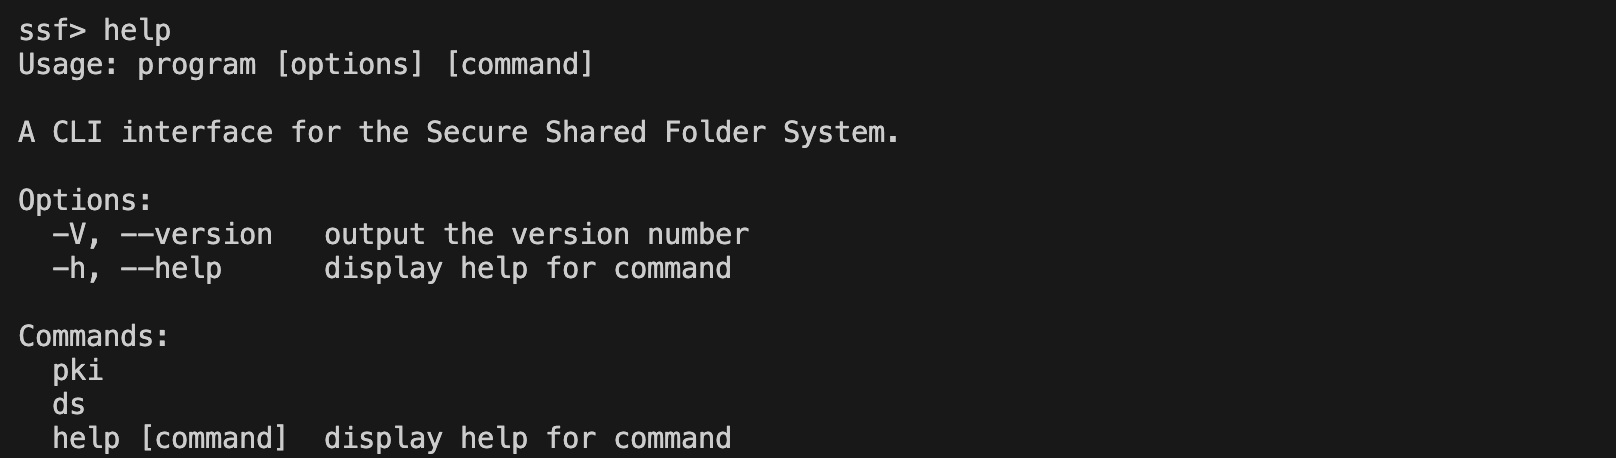
\includegraphics[width=0.8\textwidth]{figures/climain.png}
    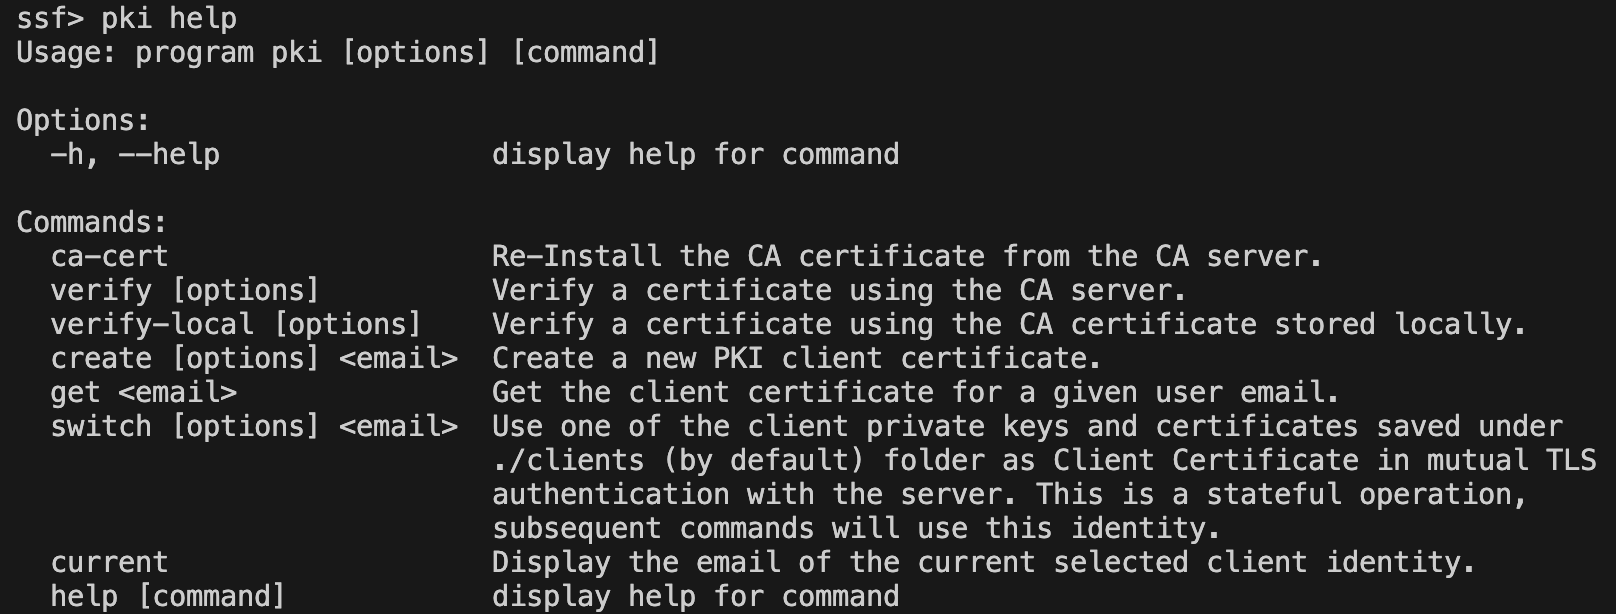
\includegraphics[width=0.8\textwidth]{figures/pkimain.png}
    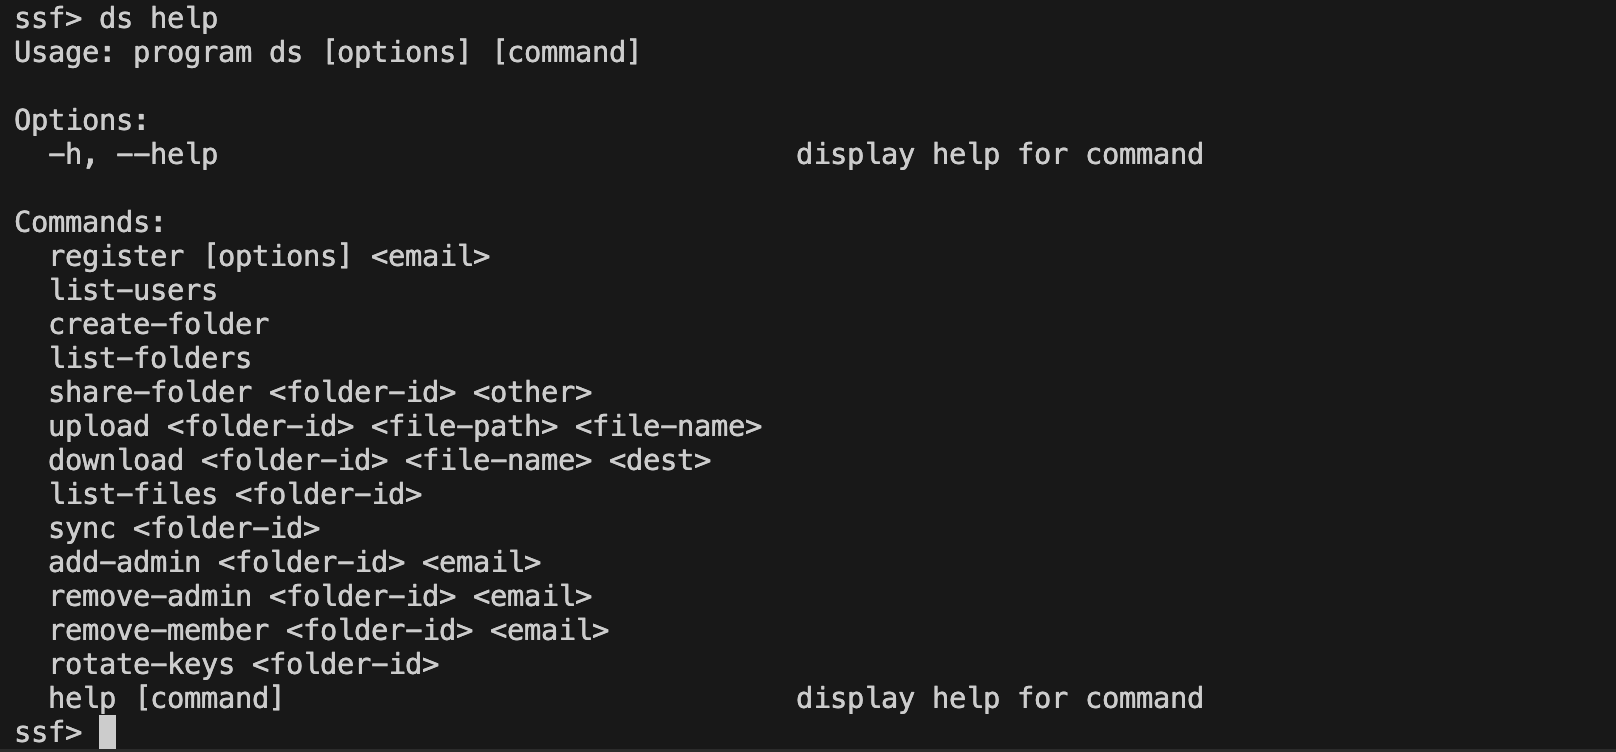
\includegraphics[width=0.8\textwidth]{figures/dsmain.png}
    \caption{CLI commands}
    \label{fig:climain}
\end{figure}

We remind the reader that some advanced functionalities
are not implemented in the baseline, therefore  
admin related commands from the ``ds'' subcommand group
return an error if the baseline protocol is used.

\paragraph{Interactive Mode}
We build the CLI interactivity using
\texttt{node:repl} module from Node.js.
The user has access to a shell-like environment
which provides command history out of the box.
The CLI can be configured to use either the
baseline protocol (\cref{ch:baseline}) or the
SSF protocol (\cref{ch:ssf}) through the environment
variable \texttt{PROTOCOL}.

\paragraph{State Management}
The baseline implementation is stateless apart
from the user identity private key, which are
stored locally in the filesystem.
The SSF implementation is stateful,
as it stores locally the cryptographic state
associated with each shared folder.
Due to library limitations explained in \cref{sc:js-bindings-for-mls}, 
we are not able to entirely persist the state of the client between invocations
when running the SSF protocols. This issue will be
fixed in future releases of the client.
For now, the CLI should be used in the interactive mode,
to maintain the client state between calls.

\subsection{Web App Setup}
The folder \texttt{www} showcases the setup
of the web application. The application is not
yet implemented, but we leave it as a reference
and to show that all the cryptographic code
we import from Wasm modules can be used
in the browser environment as well.
Interested practicioners should check
the configuration files inside \texttt{www} folder.
To create the final JS of the application
we use \texttt{Webpack}, a popular JS bundler,
which also supports loading Wasm modules.

The possibility to test some parts of the
code directly in the browser simplified some
debugging tasks, 
such as finding the compatibility issues
we describe in \cref{sc:Web-Crypto-API-implementations:-non-standard-behaviours}.
